\section{Process' Perspective}
\label{ch:background} 

\subsection{\texttt{CI/CD} pipeline using GitHub actions}
%A complete description of stages and tools included in the CI/CD chains, including deployment and release of your systems.
Our \texttt{CI/CD} pipeline is shown in Figure \ref{fig:activity_diagram}, which illustrates the process 
of creating a ticket about a feature or an issue,
developing the feature or fixing the issue, creating a pull request (\texttt{PR}),
reviewing the \texttt{PR}, merging it into the \texttt{main} branch, and finally releasing and deploying the application.
\begin{figure}[h]
      \centering
      \makebox[\linewidth]{
      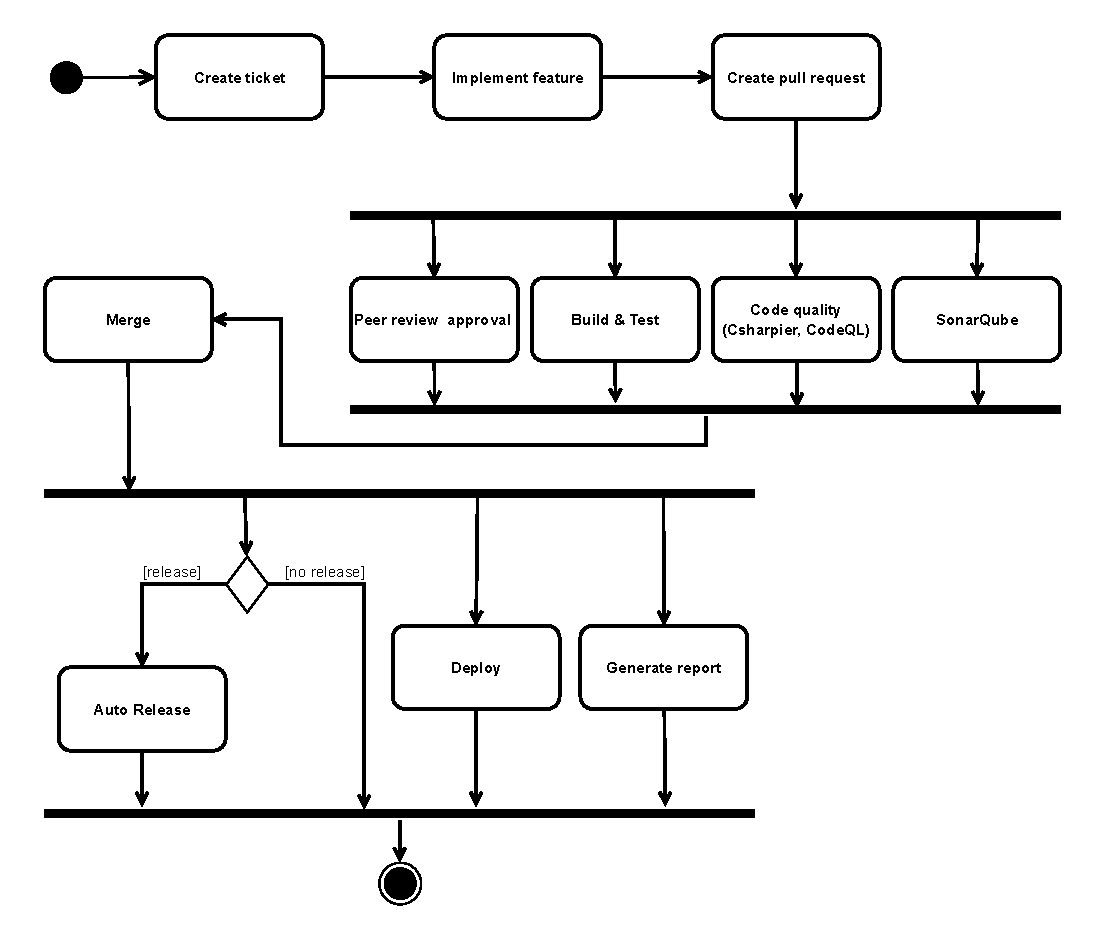
\includegraphics[width=1.4\textwidth]{images/activity_diagram.drawio.pdf}}
      \caption{Activity diagram of the CI/CD pipeline}
      \label{fig:activity_diagram}
\end{figure}

We use \texttt{GitHub} issues to create tickets for new features and issues.
The \texttt{CI/CD} pipeline is implemented using \texttt{GitHub Actions} to automate the
building, testing, analysis of code quality, releasing, and deployment
of the \texttt{MiniTwit} application.
The pipeline consists of multiple workflows: \texttt{build-test.yml}, \texttt{codeql.yml}, \texttt{auto-merge-dependabot.yml}, \texttt{auto-release.yml}, and \texttt{deploy.yml}. 
Workflows are located at \texttt{.github/workflows} in the repository.

\subsubsection{Build and Test Workflow}
This workflow is triggered on every \texttt{PR} to \texttt{main}.
The purpose of this is to build the application, run unit tests, 
and generate/upload a code coverage report.
Passing this workflow is a requirement for merging \texttt{PR}'s into \texttt{main}.

\subsubsection{Code Quality Workflow}
This workflow makes use of \texttt{GitHub}'s \texttt{CodeQL} to perform static code analysis 
of \texttt{C\#} code only.
This workflow uses the same triggers as the build and test workflow; however, 
it is also triggered on a schedule, which is set to run every \texttt{Tuesday} via a \texttt{CRON} job.
Before performing the analysis, it formats the \texttt{C\#} code using \texttt{csharpier} to 
ensure consistency and automatically commits and pushes formatting changes.
It then performs a semantic code analysis to find security vulnerabilities and 
automatically uploads the results to \texttt{GitHub}, which are displayed on \texttt{PR}'s.
This became very relevant when it once discovered that we leaked a third-party 
\texttt{API} key in our code, which we then removed and updated.

Additionally, we use \texttt{SonarQube}, \texttt{CodeFactor}, and \texttt{OpenSSF} to perform code analysis 
such as code coverage, duplication, security risks, and other best practices.
\texttt{SonarQube}'s analysis is done by using \texttt{sonarcloud-github-action}, which 
uploads the results to \texttt{SonarCloud}, and is displayed on the \texttt{PR}.
\texttt{CodeFactor} and \texttt{OpenSSF} have read access to our repository and automatically 
perform code analysis whenever our repository is updated.
The updated results are displayed on the front page of the repository on \texttt{GitHub} as badges.

\subsubsection{Auto Merge Dependabot Workflow}
Our project uses \texttt{dependabot} to automatically update dependencies in the project.
We have a \texttt{GitHub Action} that detects \texttt{PR}'s created by \texttt{dependabot}, and automatically merges 
them into \texttt{main} if all workflows pass.
This was done to ensure that we always have the latest dependencies,
and to avoid having to manually merge \texttt{dependabot} \texttt{PR}'s.

\subsubsection{Auto Release Workflow}
This workflow was inspired by a \texttt{GitHub Actions} auto release template\cite{auto-release}.
It is triggered on every push to the \texttt{main} branch, and automatically 
creates a new release on \texttt{GitHub}.
It requires a commit containing a message in the format \texttt{Release: x.y}, 
where \texttt{x} and \texttt{y} are the major and minor version numbers, respectively.
To add title and release note information, this is added to the file \texttt{CHANGELOG.md}.
The purpose of this is to automate the release process, replacing the process 
of manually creating a release on \texttt{GitHub} every time we want to release a new version 
of the application.

\subsubsection{Deployment Workflow}
This workflow is triggered on successful completion of the build and test workflow 
after a push to \texttt{main}.
It is responsible for building \texttt{Docker} images, uploading, and deploying them to 
\texttt{DigitalOcean} droplets.
To deploy, it uses \texttt{Docker Hub} to authenticate and push the built images.
It uses \texttt{scp} and \texttt{ssh} to copy two remote files \texttt{deploy.sh} 
and \texttt{docker-compose.yml} to the relevant droplet,
which are then executed to deploy the application.
For deployment safeguards; \texttt{SSH} keys, \texttt{IP} addresses, and credentials are stored in \texttt{GitHub Secrets},
which are then used in the workflows to access the \texttt{DigitalOcean} droplets and to 
authenticate with \texttt{Docker Hub}.


\subsection{Terraform}
\texttt{Terraform} is used to provision and manage our infrastructure as code, 
to automatically set up droplets in \texttt{DigitalOcean}. 
The result of the \texttt{Terraform} setup is illustrated 
in Figure \ref{fig:deployment_diagram}.
\texttt{Terraform} creates all droplets with \texttt{SSH} keys and files.
It also configures the \texttt{Docker Swarm} for the \texttt{API}.
It then calls the deploy scripts on each droplet.
Finally, it assigns the reserved \texttt{IP}'s.

To maintain infrastructure consistency and avoid creating duplicate droplets,
the \texttt{Terraform} state file is shared in a remote \texttt{DigitalOcean Spaces}.

\subsection{Logging and monitoring}
\texttt{Serilog} is used for logging \texttt{API} requests, responses, and errors.
Together with \texttt{Seq}, we can view the logs in a web interface to monitor 
application activity and display graphs containing application performance 
for developers and business statistics for stakeholders.
In \texttt{Seq}, we have three dashboards: \texttt{overview}, \texttt{endpoint overview}, and \texttt{business}.
The \texttt{overview} dashboard contains a general view of the application 
errors/exceptions and the total number of events.
The \texttt{endpoint overview} dashboard contains a view of the \texttt{API} endpoints,
showing the number of requests and average response times.
Lastly, the \texttt{business} dashboard contains a view of user activity,
showing when and how often users post tweets, and the total number of tweets over time.


\subsection{Security assessment}
To analyse security risks in our code, we use tools like \texttt{GitHub}'s \texttt{CodeQL}\cite{codeql} that 
integrate with our \texttt{CI/CD} pipeline.
This provides a display of security vulnerabilities in our code,
which is shown on the \texttt{PR}'s.

To analyse security risks of the droplets, \texttt{Docker Scout} has been used to get
quick overviews of security risks from our \texttt{Docker} images.
It scores the images in four levels: \texttt{low}, \texttt{medium}, \texttt{high}, and \texttt{critical}.
Additionally, it provides recommendations on how to fix the issues.

Additionally, we use a risk assessment matrix to assess the probability and impact of security risks. 
These are split into: probability (\texttt{unlikely}, \texttt{possible}, \texttt{likely}) and impact (\texttt{negligible}, \texttt{moderate}, and \texttt{catastrophic}).

For details about each risk scenario see Appendix \ref{appn:B}.

\subsection{Scaling}
The \texttt{Client} uses Blazor WebAssembly (\texttt{WASM}) for client-side redering, avoiding server-side 
HTML rendering.
Instead the application logic is executed in the browser, and only lightweight 
\texttt{JSON} requests are made to the \texttt{API} to fetch data.
This results in a heavly initial load, as the entire application is downloaded 
locally, however afterwards, 
this setup offers high responsiveness and scalability by addtionally using 
a \texttt{Hybrid Cache}.
To overcome the browser caching limitations (e.g. 16 GB and frequently disks 
reads), we could introduce a \texttt{Redis} cache to potentially support 
infinite and more efficient caching.

The \texttt{API} is scalable as it is stateless and uses \texttt{Docker Swarm}, 
allowing horizontal scaling of both manager and worker nodes.
With more managers we can distribute the load of incoming requests,
and with more workers we can distibute the load of processing requests.
\texttt{Database} is not currently not optimized in terms of scalability, 
as it is a single instance of \texttt{PostgreSQL}.
The Database is the bottleneck of the system, as it is the only shared 
resource between the \texttt{API}.
To fix this, we could use sharding to distribute the load of the \texttt{Database} 
across multiple instances.
By splitting the \texttt{Database} into multiple shards, we can distribute 
the load of the \texttt{API} across multiple \texttt{PostgreSQL} instances.
This could introduce some complexity and overhead, as it would be harder 
to manage and query the data.

\subsection{AI-assistants}

Gpt was of great help in translating python to csharp.
Generating files.
Not so great at ...?